

%----------------------------------------------------------------------------------------
%   PACKAGES AND OTHER DOCUMENT CONFIGURATIONS
%----------------------------------------------------------------------------------------

\documentclass[a3paper,fontscale=.9]{baposter} % Adjust the font scale/size here

\usepackage{graphicx} % Required for including images
\graphicspath{{figures/}} % Directory in which figures are stored

\usepackage{amsmath,bm} % For typesetting math
\usepackage{amssymb} % Adds new symbols to be used in math mode

\usepackage{booktabs} % Top and bottom rules for tables
\usepackage{enumitem} % Used to reduce itemize/enumerate spacing
\usepackage{palatino} % Use the Palatino font
\usepackage[font=small,labelfont=bf]{caption} % Required for specifying captions to tables and figures

\usepackage{multicol} % Required for multiple columns
\setlength{\columnsep}{1.5em} % Slightly increase the space between columns
\setlength{\columnseprule}{0mm} % No horizontal rule between columns

\usepackage{tikz} % Required for flow chart
\usetikzlibrary{shapes,arrows} % Tikz libraries required for the flow chart in the template

\newcommand{\compresslist}{ % Define a command to reduce spacing within itemize/enumerate environments, this is used right after \begin{itemize} or \begin{enumerate}
\setlength{\itemsep}{1pt}
\setlength{\parskip}{0pt}
\setlength{\parsep}{0pt}
}
\renewcommand\refname{}

\definecolor{lightred}{rgb}{0.9529,.2745,.2745} % Defines the color used for content box headers
\usepackage{lipsum}

\begin{document}

\begin{poster}
{
headerborder=closed, % Adds a border around the header of content boxes
colspacing=1em, % Column spacing
bgColorOne=white, % Background color for the gradient on the left side of the poster
bgColorTwo=white, % Background color for the gradient on the right side of the poster
borderColor=lightred, % Border color
headerColorOne=lightred, % Background color for the header in the content boxes (left side)
headerColorTwo=lightred, % Background color for the header in the content boxes (right side)
headerFontColor=white, % Text color for the header text in the content boxes
boxColorOne=white, % Background color of the content boxes
textborder=roundedleft, % Format of the border around content boxes, can be: none, bars, coils, triangles, rectangle, rounded, roundedsmall, roundedright or faded
eyecatcher=true, % Set to false for ignoring the left logo in the title and move the title left
headerheight=0.1\textheight, % Height of the header
headershape=rounded, % Specify the rounded corner in the content box headers, can be: rectangle, small-rounded, roundedright, roundedleft or rounded
headerfont=\Large\bf\textsc, % Large, bold and sans serif font in the headers of content boxes
%textfont={\setlength{\parindent}{1.5em}}, % Uncomment for paragraph indentation
linewidth=2pt, % Width of the border lines around content boxes
columns=6
}
%----------------------------------------------------------------------------------------
%   TITLE SECTION 
%----------------------------------------------------------------------------------------
%
{} % First university/lab logo on the left
{\bf\textsc{Image Regeneration with Generative Models}} % Poster title
{\textsc{ Abhijith C.(1MV14CS004), Raghava G. Dhanya(1MV14CS077) and Shashank S.(1MV14CS131)\\Guide: Sushila Shidnal\\ Sir M. Visvesvaraya Institute of Technology }} % Author names and institution
{}% {\includegraphics[height=4em]{example-image}} % Second university/lab logo on the right



\headerbox{Abstract}{name=abstract,column=0,row=0,span=6}{
Current advances in Generative Adversarial Networks allow us to obtain near realistic images but it is still quite distinguishable from actual photographic images. The technology is also not very amiable to changes in the orientation of images in Convolutional Neural Networks(CNN). Additionally, the amount of data required to train the network must be exhaustible, for example, in case different perspectives of a face are required the various perspectives must be explicitly present in the training data to achieve the result. Thus the network requires humongous amounts of data.\par
In this project we propose a novel approach to accomplish the same results using CapsNet. CapsNet employs a dynamic routing algorithm which replaces the scalar-output feature detectors of the CNN with vector-output capsules. A capsule is essentially a group of neurons describing a specific part of object or image. Active capsules at one level make predictions, via transformation matrices, for the instantiation parameters of higher-level capsules. In essence, the CapsNet is the reverse of the common Computer Graphics pipeline where we convert objects to their renders. The CapsNet works from the pixel level and works up towards the object.
}



\headerbox{Generative Adversarial Networks}{name=gan,below=abstract,span=3}{
Generative Adversarial Networks\cite{gan} pose the training process as a game between two distinct networks: A neural network, called the generator, generates new instances of data, while the another, the discriminator, evaluates their authenticity; Discriminator network tries to classify samples as either coming from the true distribution $p(x)$ or the model distribution $\hat{p}(x)$. Every time the discriminator notices a difference between the two distributions, the feedback is given to the generator and the generator adjusts its parameters slightly to make it go away, until at the end (in theory) the generator exactly reproduces the true data distribution and the discriminator is guessing at random, unable to find a difference.\par
\begin{center}
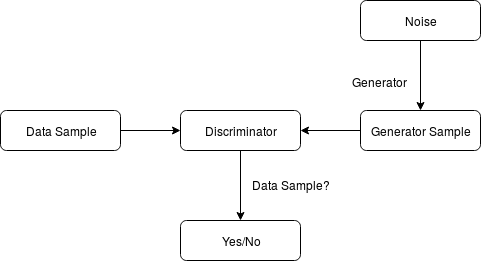
\includegraphics[width=.8\textwidth]{vanillaGAN.png}\par
\end{center}

\noindent This can be represented in the form of a minimax game \\
\begin{equation} \label{eu_eqn}
\min_{G} \max_{D} V(D, G)=\mathbb{E}_{\bm{x} \sim p_{\text{data}}(\bm{x})}[\log D(\bm{x})]+\mathbb{E}_{\bm{z} \sim p_{\bm{z}}(\bm{z})}[\log (1 - D(G(\bm{z})))]
\end{equation}
}

\headerbox{Capsule Networks}{name=caps,below=abstract,span=3,column=3}{
A capsule is a nested set of neural layers. Capsules are like cortical columns in human brains. Deep neural nets learn by back-propagation of errors over the entire network. In contrast, human brains supposedly wire neurons as explained by the Hebbian Theory: "units that fire together, wire together".\par Capsules mimic Hebbian learning in the way that: "A lower-level capsule prefers to send its output to higher level capsules whose activity vectors have a big scalar product with the prediction coming from the lower-level capsule". A combination of capsules encode objects' parts AND their relative positions, so an object instance can be accurately derived from the presence of the parts at the right locations, and not just their presence. Capsules produce equivariant features. Capsules predict the activity of higher-layer capsules to route information to the right higher-layer capsules, a process called "Dynamic routing"\cite{capsnet}.
}

\headerbox{Results 1}{name=results1,below=gan,column=0,span=3}{

    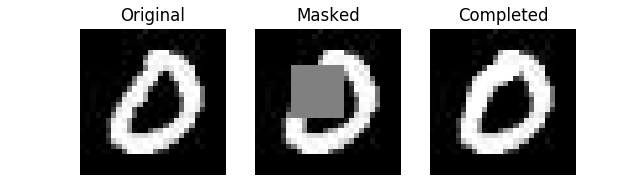
\includegraphics[width=.5\linewidth]{completion_outputs/0_1.png} 
    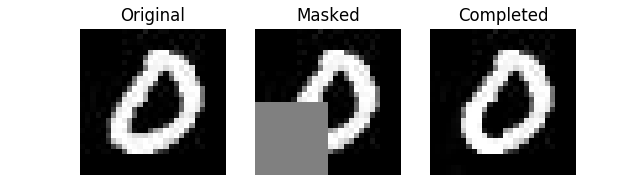
\includegraphics[width=.5\linewidth]{completion_outputs/0_2.png} 
    \\
    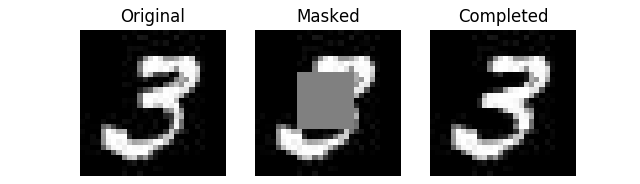
\includegraphics[width=.5\linewidth]{completion_outputs/3_1.png}
    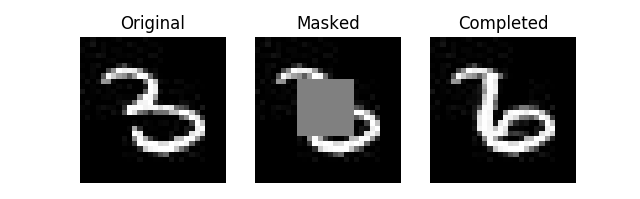
\includegraphics[width=.5\linewidth]{completion_outputs/3_2.png}
    \\
    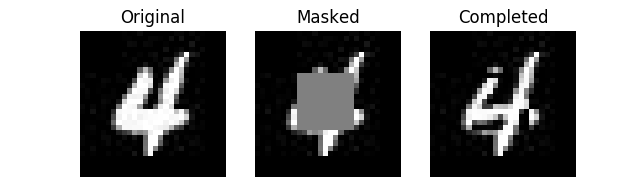
\includegraphics[width=.5\linewidth]{completion_outputs/4.png}
    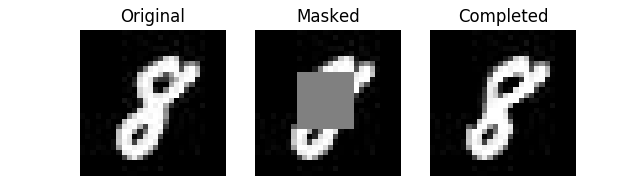
\includegraphics[width=.5\linewidth]{completion_outputs/8_1.png}

\begin{center}
    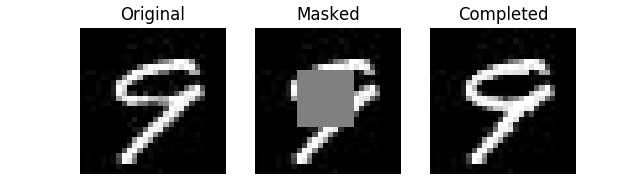
\includegraphics[width=.5\linewidth]{completion_outputs/9_1.png} 
\end{center}
    
}

\headerbox{Semantic Inpainting}{name=inpainting,below=caps,span=3,column=3}{
Inpainting is the process of reconstructing lost or deteriorated parts of images and videos. In the museum world, in the case of a valuable painting, this task would be carried out by a skilled art conservator or art restorer. In the digital world, inpainting (also known as image interpolation or video interpolation) refers to the application of sophisticated algorithms to replace lost or corrupted parts of the image data (mainly small regions or to remove small defects). As a demonstration of the application of our modified GAN, we use Semantic Inpainting. A part of the image is obscured by a mask. When this image is passed to the network, it reconstructs the image by filling in the mask.

}

\headerbox{Results 2}{name=results2,below=inpainting,column=3,span=3}{
    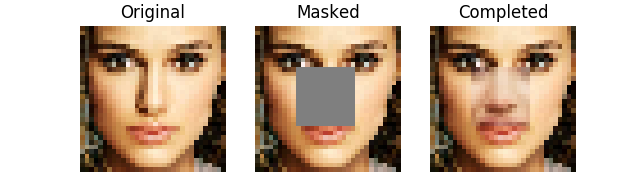
\includegraphics[width=.5\linewidth]{completion_outputs/Figure_1.png}
    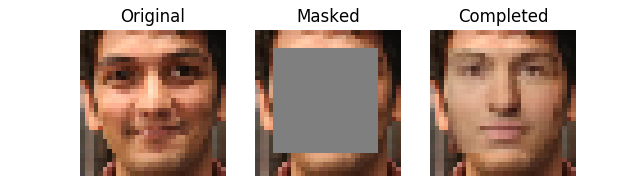
\includegraphics[width=.5\linewidth]{completion_outputs/Figure_2.png} 
    \\
    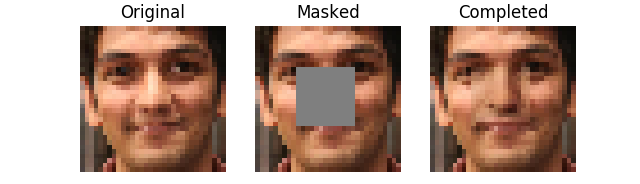
\includegraphics[width=.5\linewidth]{completion_outputs/Figure_3.png}
    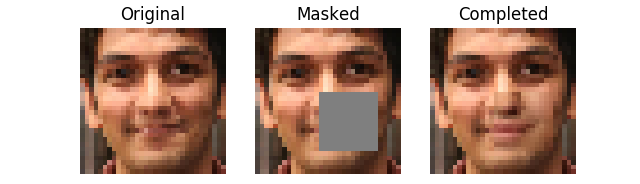
\includegraphics[width=.5\linewidth]{completion_outputs/Figure_4.png}
    \\
    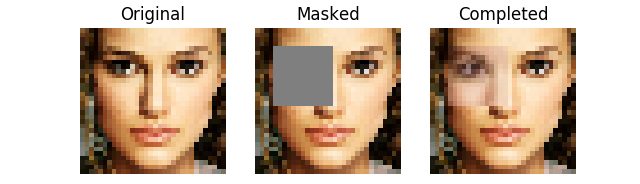
\includegraphics[width=.5\linewidth]{completion_outputs/Figure_14.png}
    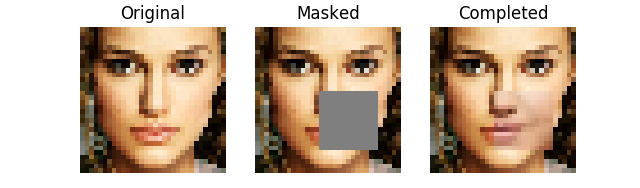
\includegraphics[width=.5\linewidth]{completion_outputs/Figure_15.png}
    
\begin{center}
    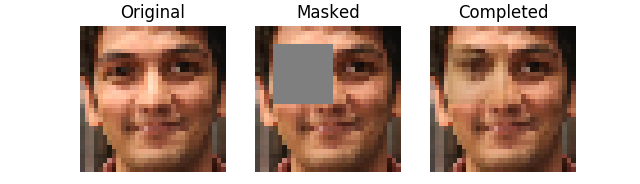
\includegraphics[width=.5\linewidth]{completion_outputs/Figure_5.png}
\end{center}
}

%----------------------------------------------------------------------------------------
%   REFERENCES
%----------------------------------------------------------------------------------------

\headerbox{References}{name=references,column=0,span=3,below=results1}{
\bibliography{ref}{}
\bibliographystyle{plain}

}


\headerbox{Conclusion}{name=conclusion,column=3,span=3,aligned=references,below=results2}{ % This block is as tall as the references block
During the course of this project, we wished to replicate the results of the existing state-of-the-art in Generative Models and perform a comparative study. We implemented four different versions of GANs and modified them with CapsNet. Our motivation was based on the idea that CapsNet is more capable of understanding the variances in objects. This in turn should lead to lower data requirements during training of the model and consequently lower power consumption. \par
In conclusion, we can confidently state that augmenting the GANs with CapsNet was a fruitful endeavor. The CapsNet helped to reduce th training overhead considerably when compared to classical networks while providing remarkably similar results. Our research shows that embedding CapsNet into the GAN, in certain cases, improves upon its performance.
}


%----------------------------------------------------------------------------------------

\end{poster}

\end{document}\grid
